\documentclass{beamer}
\usepackage[utf8]{inputenc}
\usepackage{listings}
\usepackage{booktabs}
\usepackage{amssymb}
\usepackage{nicefrac}
\usepackage{amsmath}
\usepackage{bbm}
\usepackage{bm}
\usepackage{enumitem}
\usepackage{hyperref}
\usepackage[export]{adjustbox}
\usepackage{svg}

\usetheme{Madrid}
\definecolor{mlpblue}{rgb}{0.1, 0.14, 0.24}

\useoutertheme{infolines} % Alternatively: miniframes, infolines, split
\useinnertheme{circles}
\usecolortheme[named=mlpblue]{structure}

\DeclareMathOperator{\Tr}{Tr}
\DeclareMathOperator{\Cov}{Cov}
\DeclareMathOperator{\Concat}{Concat}

\DeclareMathOperator*{\argmax}{arg\,max}
\DeclareMathOperator*{\argmin}{arg\,min}
\DeclareMathOperator*{\indep}{\perp \!\!\! \perp}

\lstset{basicstyle=\footnotesize\ttfamily,breaklines=true}

%------------------------------------------------------------
%This block of code defines the information to appear in the
%Title page
\title[RT1, RT2, OpenVLA]{Vision-Language-Action Models}

\subtitle{RT1, RT2, OpenVLA} %\thanks{Beaglehole, Súkeník et.~al.~[NeurIPS 2024]}}
\author[MLP]{A. Buynitsky} 
\date{Jan 26, 2025}
\titlegraphic{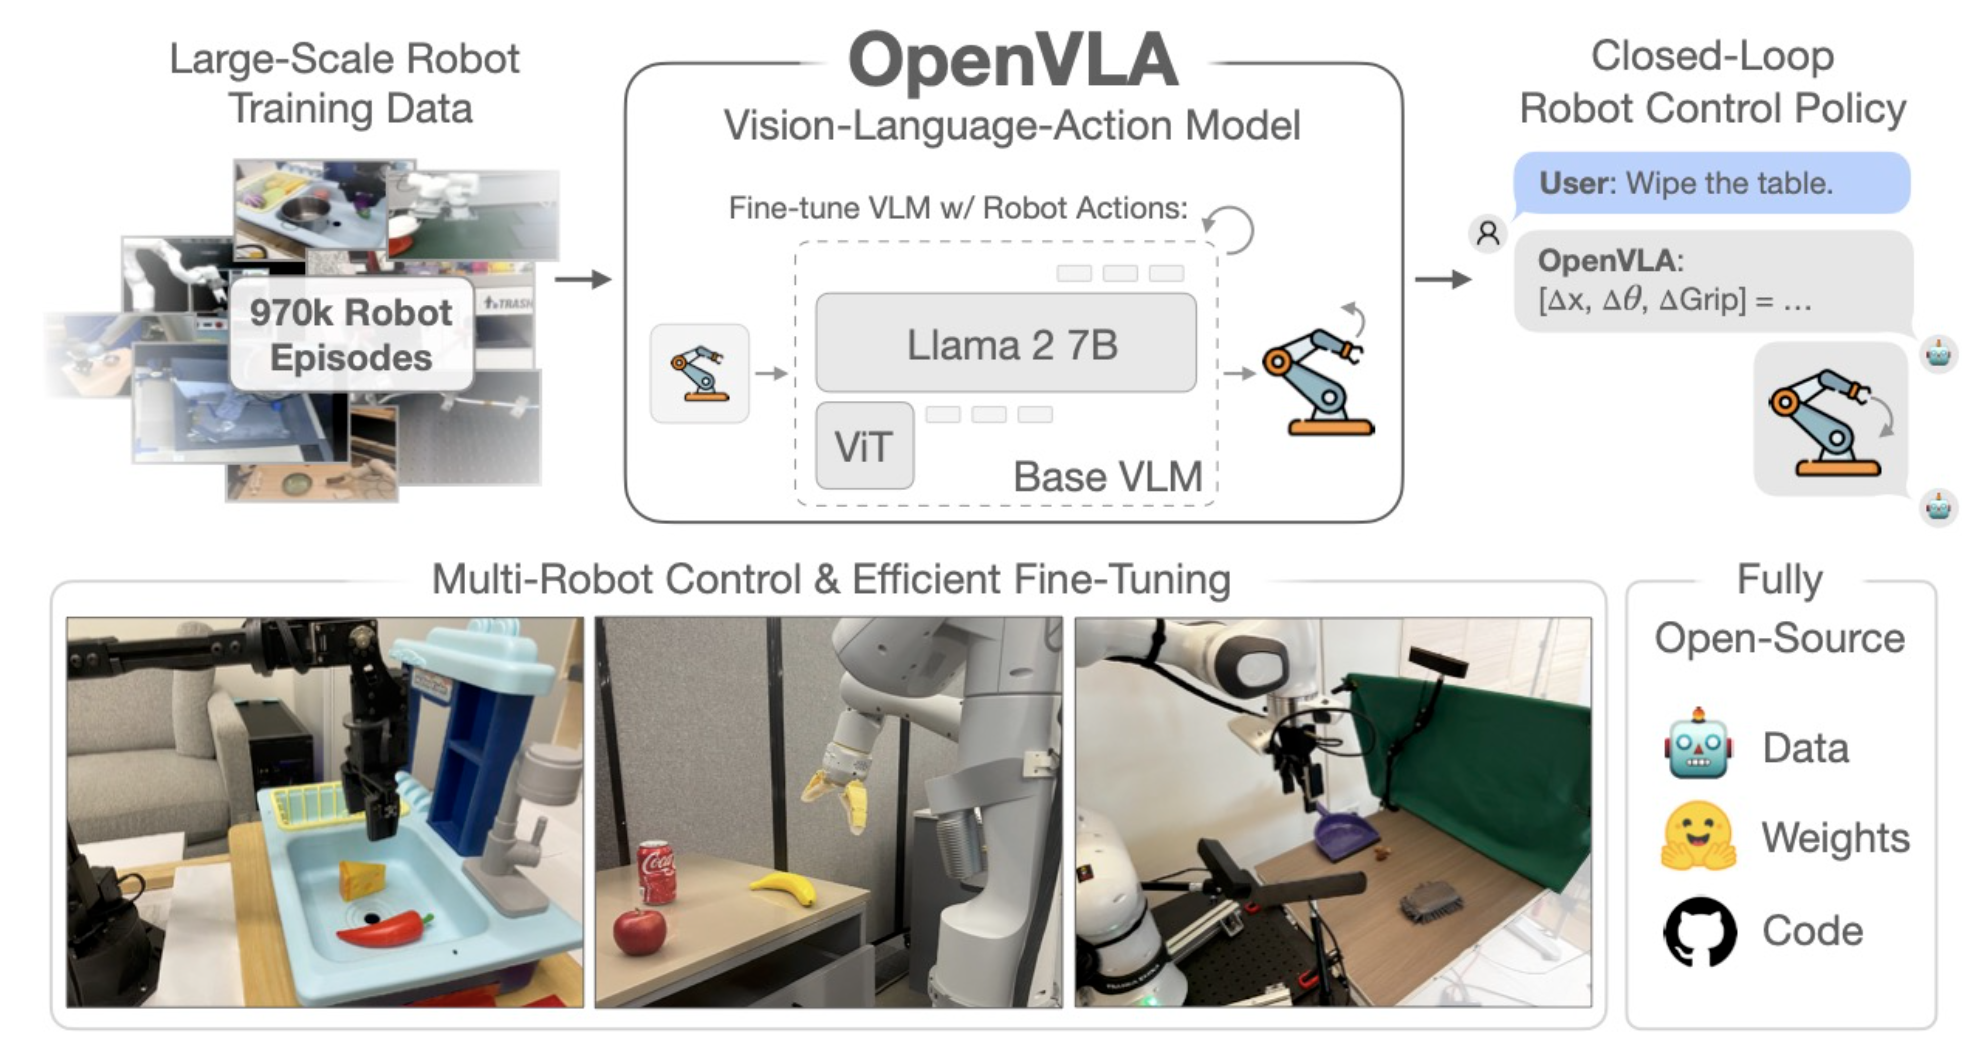
\includegraphics[width=7cm]{./img/title.png}}

%End of title page configuration block
%------------------------------------------------------------

%The next block of commands puts the table of contents at the 
%beginning of each section and highlights the current section:

\AtBeginSection[]
{
  \begin{frame}
    \frametitle{Outline}
    \tableofcontents[currentsection]
  \end{frame}
}
% ------------------------------------------------------------


\begin{document}

\frame{\titlepage}


%---------------------------------------------------------
% This block of code is for the table of contents after
% the title page
\begin{frame}
\frametitle{Outline}
\tableofcontents
\end{frame}
%---------------------------------------------------------
\section{RT1}

\begin{frame}[t]{FiLM Layers}
    FiLM adaptively influence output of neural network by applying a affine (linear) transformation to intermediate layers. \newline
    \begin{columns}
        \hspace{1em}
		\begin{column}{.5\textwidth}
            FiLM learns functions $f$ and $h$  based on external input $x_i$ (i.e image) in a batch
             % i is batch dimension in this case
            % c is cth feature dimension
            \small
                \[\gamma_{i,c} = f_c(x_i) \quad \beta_{i,c} = h_c(x_i)\]
                \[\text{FiLM}(F_{i,c} \mid \gamma_{i,c}, \beta_{i,c}) = \gamma_{i,c} F_{i,c} + \beta_{i,c}\]
            \normalsize
            $F_{i,c}$ is the $c^{th}$ feature of the $i^{th}$ sample in the batch
		\end{column}
        \hspace{0em}
		\begin{column}{.5\textwidth}
            \begin{center}
                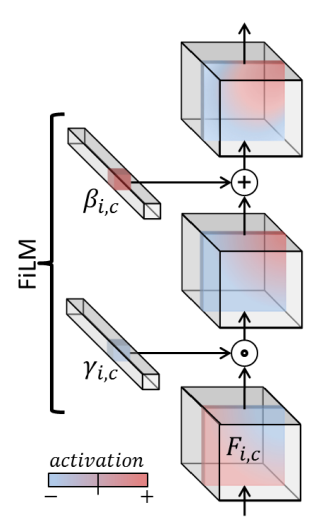
\includegraphics[width=0.6\textwidth]{./img/film_comp.png}
            \end{center}
		\end{column}
	\end{columns}
\end{frame}

\begin{frame}[t]{ \href{https://arxiv.org/pdf/1709.07871}{FiLM} Layers}
    FiLM adaptively influence output of neural network by applying a affine (linear) transformation to intermediate layers. \newline
    \begin{columns}
        \hspace{1em}
		\begin{column}{.5\textwidth}
            FiLM learns functions $f$ and $h$  based on external input $x_i$ (i.e image) in a batch
             % i is batch dimension in this case
            % c is cth feature dimension
            \small
                \[\gamma_{i,c} = f_c(x_i) \quad \beta_{i,c} = h_c(x_i)\]
                \[\text{FiLM}(F_{i,c} \mid \gamma_{i,c}, \beta_{i,c}) = \gamma_{i,c} F_{i,c} + \beta_{i,c}\]
            \normalsize
            $F_{i,c}$ is the $c^{th}$ feature of the $i^{th}$ sample in the batch
		\end{column}
        \hspace{0em}
		\begin{column}{.5\textwidth}
            \begin{center}
                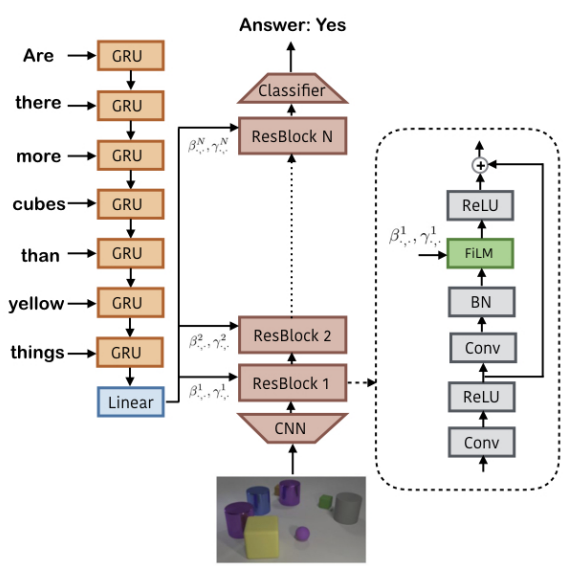
\includegraphics[width=0.8\textwidth]{./img/film_arch.png}
            \end{center}
		\end{column}
	\end{columns}
\end{frame}

\begin{frame}[t]{ \href{https://arxiv.org/pdf/2106.11297}{TokenLearner}}
    \vspace{-0.5em}
    %TokenLearner decreases number of tokens (81) into smaller amount (8).\newline
    %Address patch tokenization challenges in ViT. \newline
    \textbf{Goal:} Generate $\left[z_i\right]^S_{i=1} \in \mathbb{R}^{S \times C}$ from $x \in \mathbb{R}^{H \times W \times C}$
    by learning $S$ functions $A_i$ to adaptively select informative combo of pixels in $x_t$ denoted as:
    \[z_i = A_i(x)\]
    Implement with weight map $\alpha_i(x)$ and spatial global average pooling $\rho(x)$:
    \[z_i = A_i(x) = \rho(x \odot \gamma(\alpha_i(x)))\]
    % gamma is broadcasting function projecting to all channels
    \begin{center}
        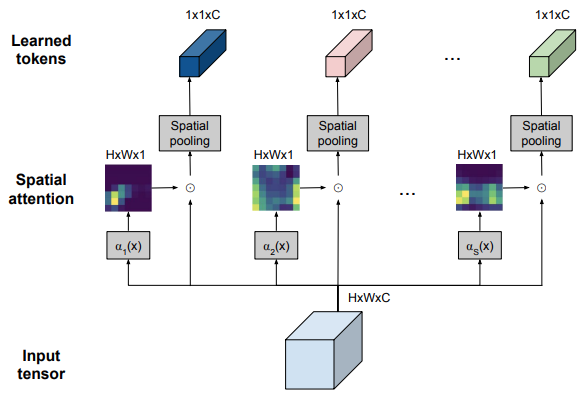
\includegraphics[width=0.55\textwidth]{./img/tokenlearner.png}
    \end{center}
\end{frame}

\begin{frame}[t]{RT1 Architecture (Part 1)}
    \begin{columns}
        \hspace{1em}
		\begin{column}{.5\textwidth}
            \begin{itemize}[label=-]
                \item  \textbf{Unversal Sentence Encoder:} Encoder block of Transformer\newline
                % encoding setnence meaning trained embedding usin other tasks ie sentiment analysis
                \item \textbf{FiLM Layers:} Conditions EfficientNet on text\newline
                % important: identity initialize film layers so that at start of training is just pretrained img net
                \textbf{TokenLearner:} Donwsample 81 to 8 tokens per image \newline
                \item \textbf{Transformer:} Apply transformer to FiLM output\newline
            \end{itemize}
		\end{column}
        \hspace{0em}
		\begin{column}{.5\textwidth}
            \begin{center}
                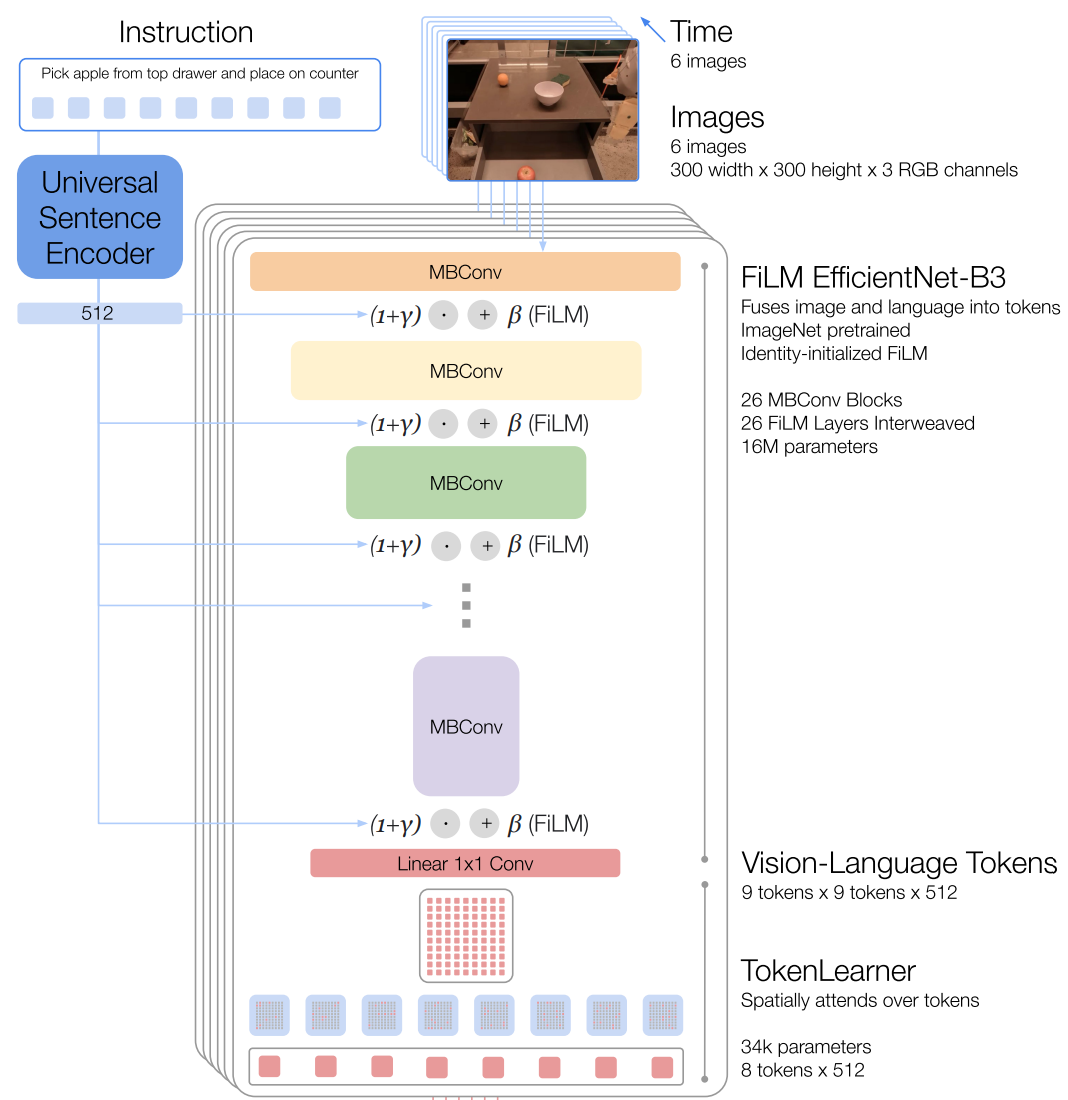
\includegraphics[width=1.0\textwidth]{./img/rt1_arch.png}
            \end{center}
		\end{column}
	\end{columns}
\end{frame}

\begin{frame}[t]{RT1 Architecture (Part 2)}
    \begin{columns}
        \hspace{0.5em}
		\begin{column}{.5\textwidth}
            \begin{itemize}[label=-]
                \item \textbf{History:} 6-image history for total of 48 tokens
                \item \textbf{Transformer:} decoder-only arch with 8 self-attn layers
                \item \textbf{Action Tokenization:} Discretize continuous actions to 256 bins:
                \begin{itemize}[label=-]
                    \item \textbf{Gripper Actions:} $x,y,z,\rho,\phi,\theta$, opening of gripper
                    % output: lenght 11 sequence with possible 256 tokens
                    % have a cross-entropy loss for training
                    \item \textbf{Base Actions:} $x,y$ head angle
                    \item \textbf{mode:} control arm, control base or terminate
                \end{itemize}
            \end{itemize}
		\end{column}
        \hspace{0em}
		\begin{column}{.5\textwidth}
            \begin{center}
                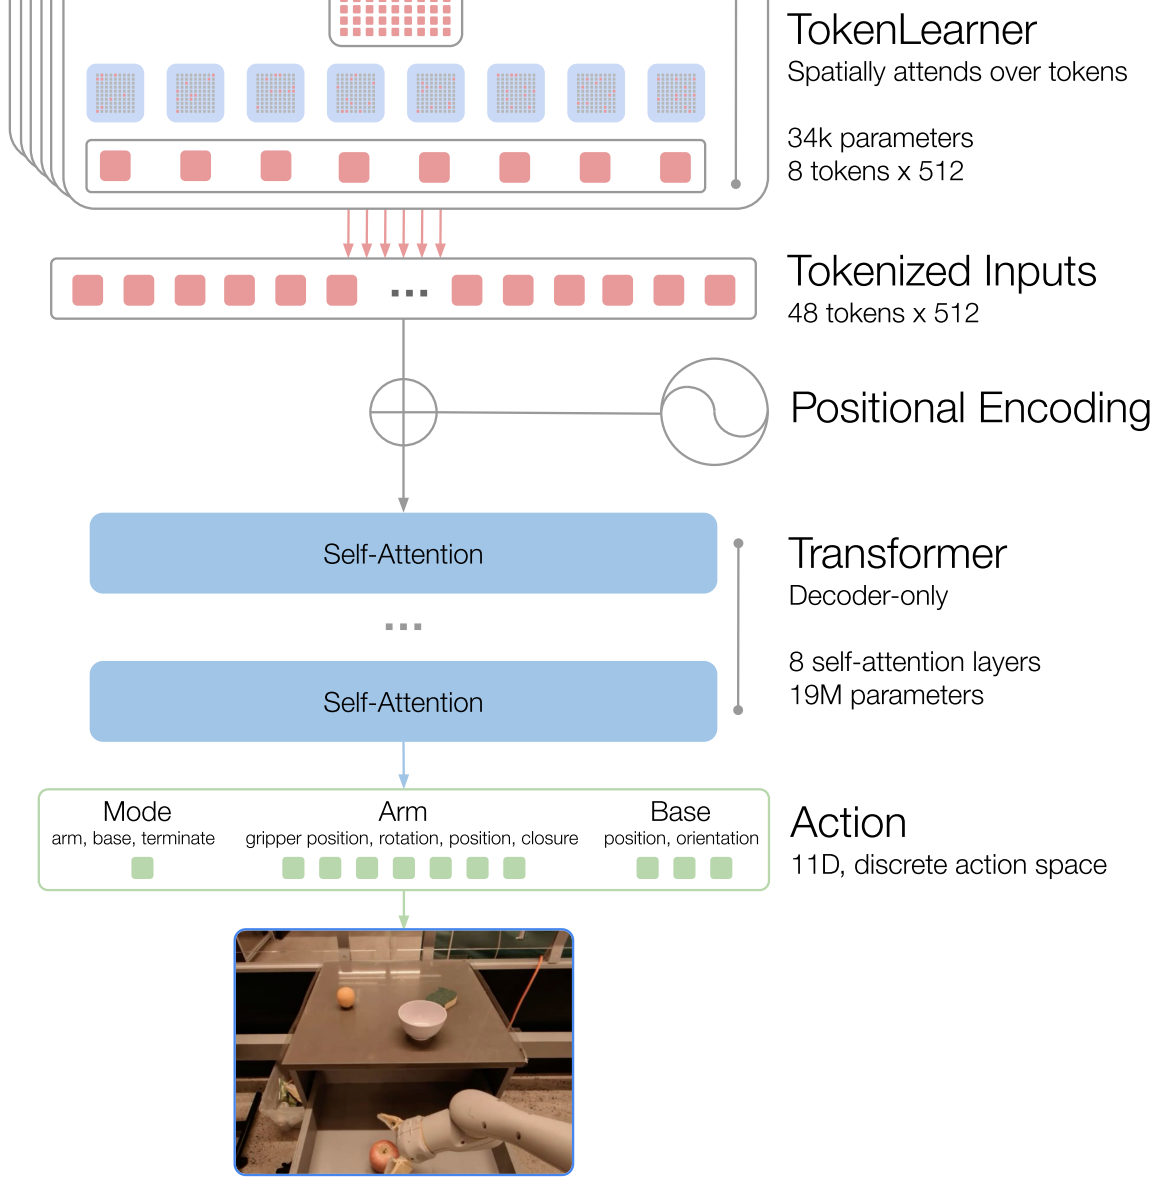
\includegraphics[width=1.0\textwidth]{./img/rt1_arch_2.png}
            \end{center}
		\end{column}
        \hspace{0.25em}
	\end{columns}
\end{frame}

\section{RT2}

\begin{frame}[t]{Converting VLMs to VLAs}
    \textbf{Goal:} Associate actions from model's existing tokenization for: \newline
    \[\text{terminate } \Delta \text{pos}_x \, \Delta \text{pos}_y \, \Delta \text{pos}_z \, \Delta \text{rot}_x \, \Delta \text{rot}_y \, \Delta \text{rot}_z \, \text{gripper\_extension}\]
    Possible instantiation: "1 128 91 241 5 101 127" \newline
    % lie before Discretize continuous actions to 256 bins. \newline
    \newline
    \textbf{PaLI-X Tokenization:} Integers up to 1000 each have unique token, so associate action bins to token corresponding to integer \newline  
    \textbf{PaLM-E Tokenization:} Overwrite the 256 least frequently used tokens to represent action vocabulary.
    \newline
    \textbf{Co-Fine-Tuning:} Train with both robotics data "Q: what action should robot take to [task instruction]? A:" and original web data. \newline
    % co-fine-tuning: balance rations of robot and web data in each training batch
    % increase sampling weighton robt dataset over time
    % policy explsoed to both abstract visual concepts from web dat and low-level robotic actions
    % only constrain to sample output 
\end{frame}

\begin{frame}[t]{RT2 Architecture}
    % \begin{center}
    %     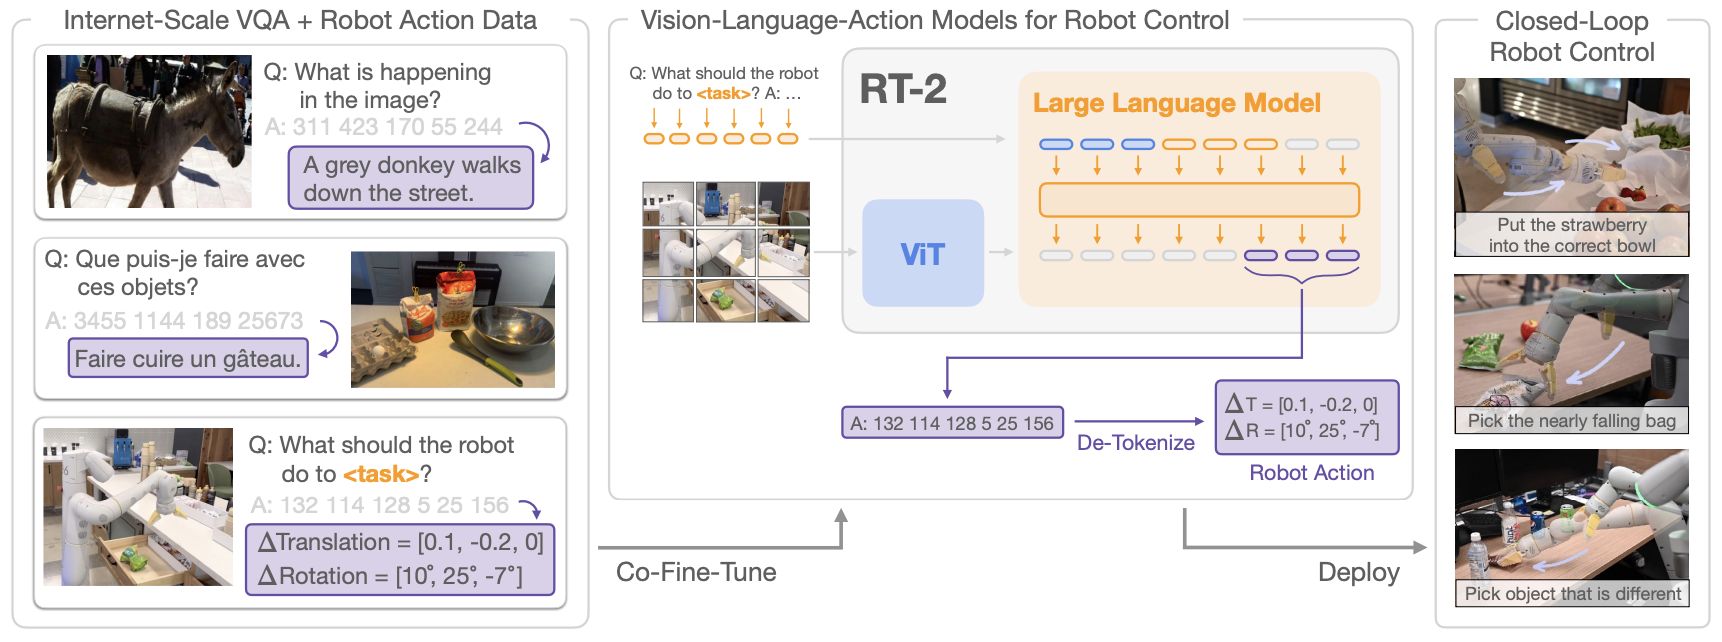
\includegraphics[width=0.8\textwidth]{./img/rt2.png}
    %     % start out with mixed data
    %     % then take image, patchify (spllit 16x16 patches)
    %     % then feed to Palm and get action tokens with history 
    % \end{center}
    \textbf{Prefix-decoder-only LLMs:} \newline
    LLM is auto-regressive: condition model on prompt (prefix $w_{1:n}$) consisting of token embeddings $w_i \in \mathcal{X} \subset \mathbf{R}^k$: \newline
    \[p(w_{n+1:L} \mid w_{1:n}) = \prod_{l=n+1}^{L} p_{\text{LM}}(w_l \mid w_{1:l-1})\]
    Train end-to-end embeddings $\gamma: \mathcal{W} \rightarrow \mathcal{X}$:
    \[x_i = \gamma(w_i),\]
    \textbf{Adding Images:} \newline
    ViT maps image $I$ to tokens $\tilde{x}_{1:m} = \tilde{\phi}_{\text{ViT}}(I) \in \mathbf{R}^{m \times \tilde{k}}$\newline
    Project $\tilde{x}_{1:m}$ to embedding space via affine transformation $\psi: \mathbf{R}^{\tilde{k}} \rightarrow \mathbf{R}^k$\newline

    \textbf{Robot State:} (Joint angles, gripper state, etc.) \newline
    Project $s \in \mathbf{R}^S$ to embedding space via affine transformation $\psi: \mathbf{R}^S \rightarrow \mathbf{R}^k$\newline
\end{frame}

\begin{frame}[t]{RT2 Architecture and Results}
    \textbf{Complete Architecture:}
    \begin{center}
        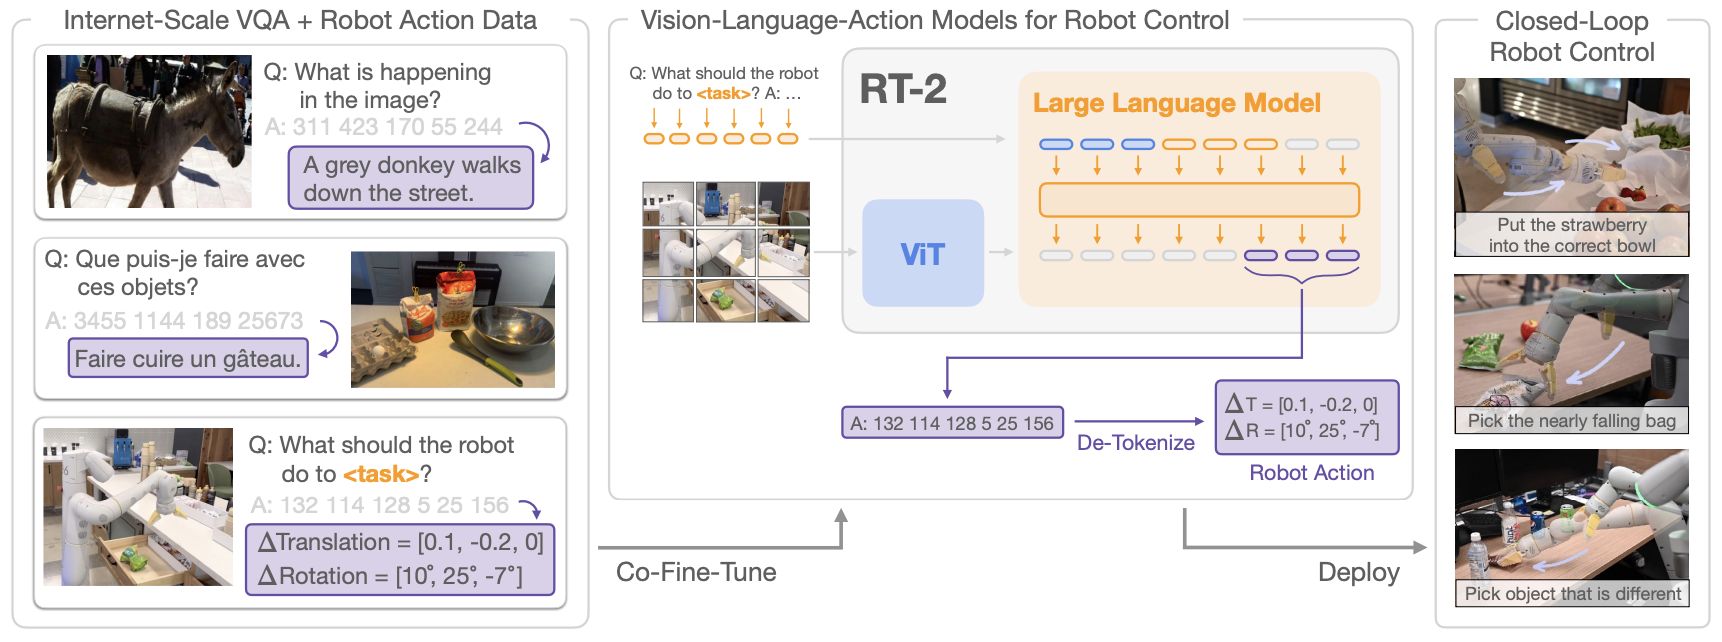
\includegraphics[width=0.8\textwidth]{./img/rt2.png}
        % start out with mixed data
        % then take image, patchify (spllit 16x16 patches)
        % then feed to Palm and get action tokens with history 
    \end{center}
    \textbf{Results:}
    \begin{center}
        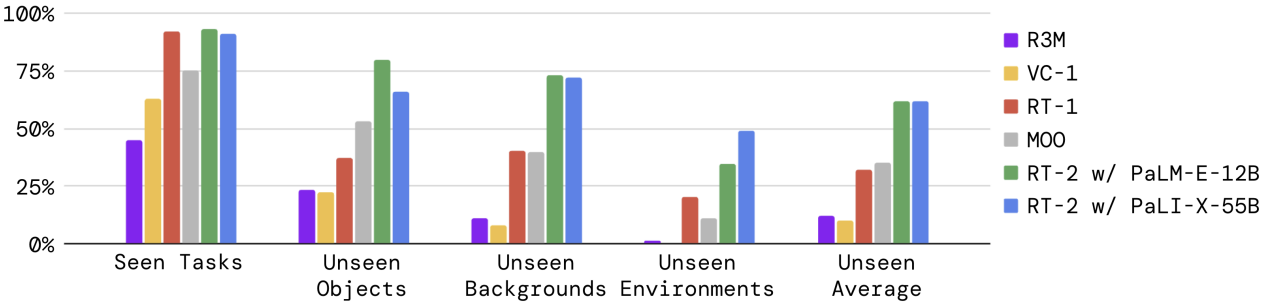
\includegraphics[width=0.8\textwidth]{./img/rt2_results.png}
    \end{center}
\end{frame}

\section{OpenVLA}
\begin{frame}[t]{OpenVLA Architecture}
    \textbf{Complete Architecture:}
    \begin{center}
        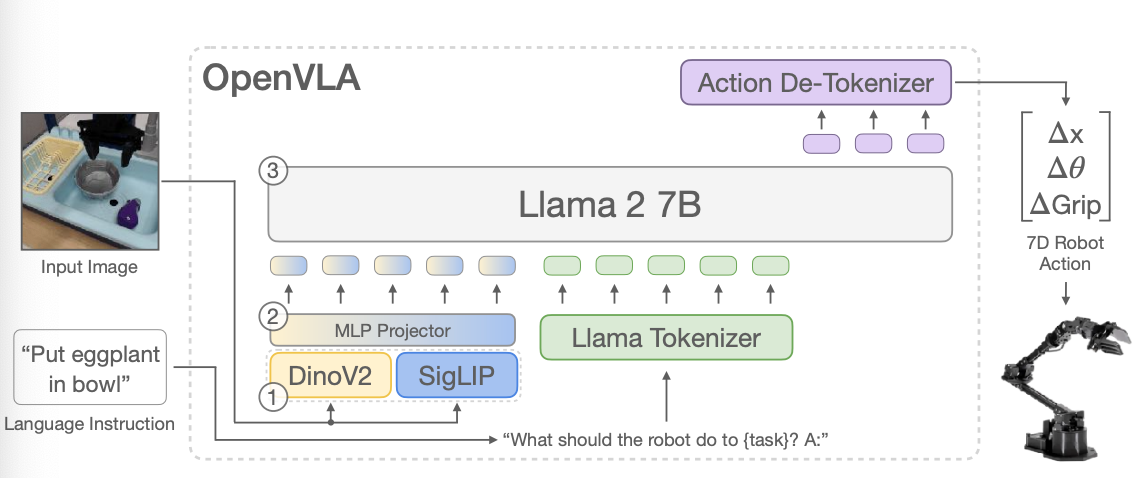
\includegraphics[width=0.8\textwidth]{./img/openvla_arch.png}
    \end{center}
    \begin{columns}
        \hspace{0.5em}
		\begin{column}[t]{.33\textwidth}
            \textbf{Vision Encoder:}\newline
            \small
            Concatenate embeddings from SigLip and DinoV2 channelwise
            % found that dinov2 has better spatial understnading tha siglip
		\end{column}
        \hspace{0em}
		\begin{column}[t]{.33\textwidth}
            \textbf{Projection Layer}\newline
            \small
            2-layer MLP projecting to embedding dimension of llama (512)
		\end{column}
        \hspace{0.25em}
		\begin{column}[t]{.33\textwidth}
            \textbf{LLM Backbone:}\newline
            \small
            Llama-2 7B
		\end{column}
	\end{columns}
\end{frame}

\begin{frame}[t]{Data and Tokenization Details}
    \textbf{Tokenizer}
    \begin{itemize}[label=-]
        \item LLama tokenizer reserves 100 toeksn for fine-tuning.
        \item Chose to follow RT2 tokenization. Discretize each dim of robot actions seperately into one of 256 bins.
        \item Replace 256 least frequent tokens with action tokens.
    \end{itemize}
    \textbf{Training Data}
    \begin{itemize}[label=-]
        \item OpenX dataset (70 robot embeddings w/ > 2M trajectories)
        \item Restrict datasets to contain only 1 manipulator with 3rd pov camera
        \item weight down / remove less diverse datasets, up-weight datasets with larger task and scene diversity
    \end{itemize}
\end{frame}

\begin{frame}[t]{Training Details}
    \begin{itemize}[label=-]
        \item Decrease image resolution from $384 \times 384$ to $224 \times 224$ for $3\times$ training speedup
        % before had vision encoder frozen during training
        \item Train until accuracy passes 95\% (27 epochs using fixed lr of 2e-5)
        % found no performance decrease here
        \item finetune vision encoder weights for better spatial understanding
        \item Train on 64 A100 GPUs for 14 days using batch size of 2048
        \item requires 15GB of GPU memory when loading in bfloat16
    \end{itemize}
\end{frame}
\begin{frame}[t]{Fine-Tuning OpenVLA}
    \begin{itemize}[label=-]
        \item \textbf{full finetune:} updats all weights during training
        \item \textbf{last layer only:} finetunes only last layer of transformer backbone and embedding matrix
        \item \textbf{sandwich} finetunes vision encoder, embedding matrix and last layer 
        \item \textbf{LoRA} applied to all layers of the model using varying rank $r \in {32, 64}$
    \end{itemize}
    \begin{center}
        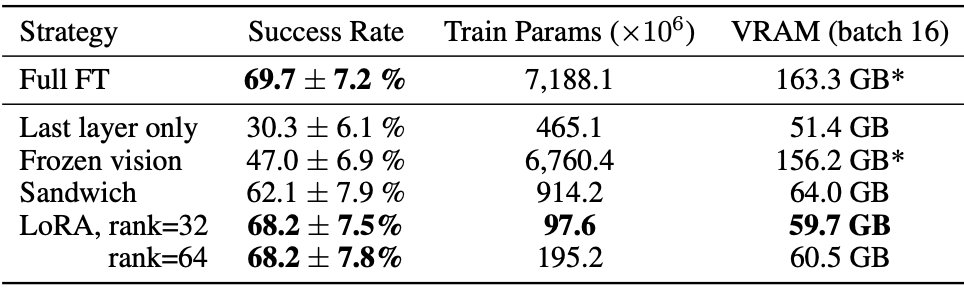
\includegraphics[width=0.8\textwidth]{./img/openvla_sft.png}
    \end{center}
\end{frame}

\begin{frame}[t]{Results and Quantization}
    \textbf{Overall Results:}
    \begin{center}
        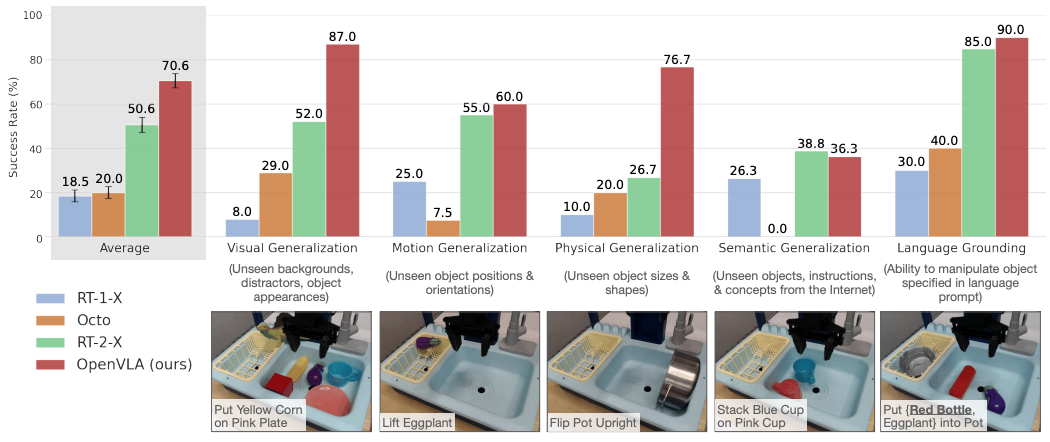
\includegraphics[width=0.8\textwidth]{./img/openvla_results.png}
    \end{center}
    \begin{columns}
		\begin{column}[t]{.33\textwidth}
            \textbf{Inference Speed:}\newline
            % 1080Ti has only 16 GB
            % ♠: Model shared across 2 GPU to fit
            \vspace{-2em}
            \begin{center}
                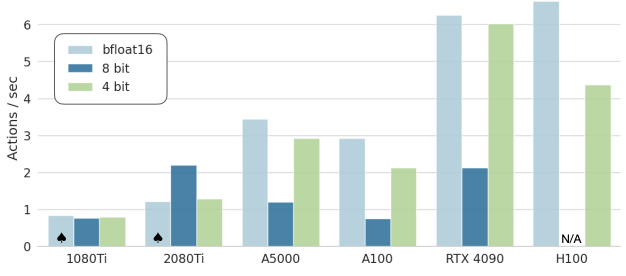
\includegraphics[width=1.2\textwidth]{./img/openvla_speed.png}
                % reduced inference speed: ob serve a decrease in performance
            \end{center}
		\end{column}
        \hspace{0em}
		\begin{column}[t]{.33\textwidth}
            \textbf{Quantization Results:}\newline
            \begin{center}
                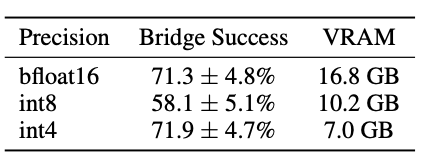
\includegraphics[width=1.0\textwidth]{./img/openvla_quant.png}
            \end{center}
		\end{column}
	\end{columns}
\end{frame}

\section{Aloha}
\begin{frame}[t]{Aloha}
    \begin{center}
        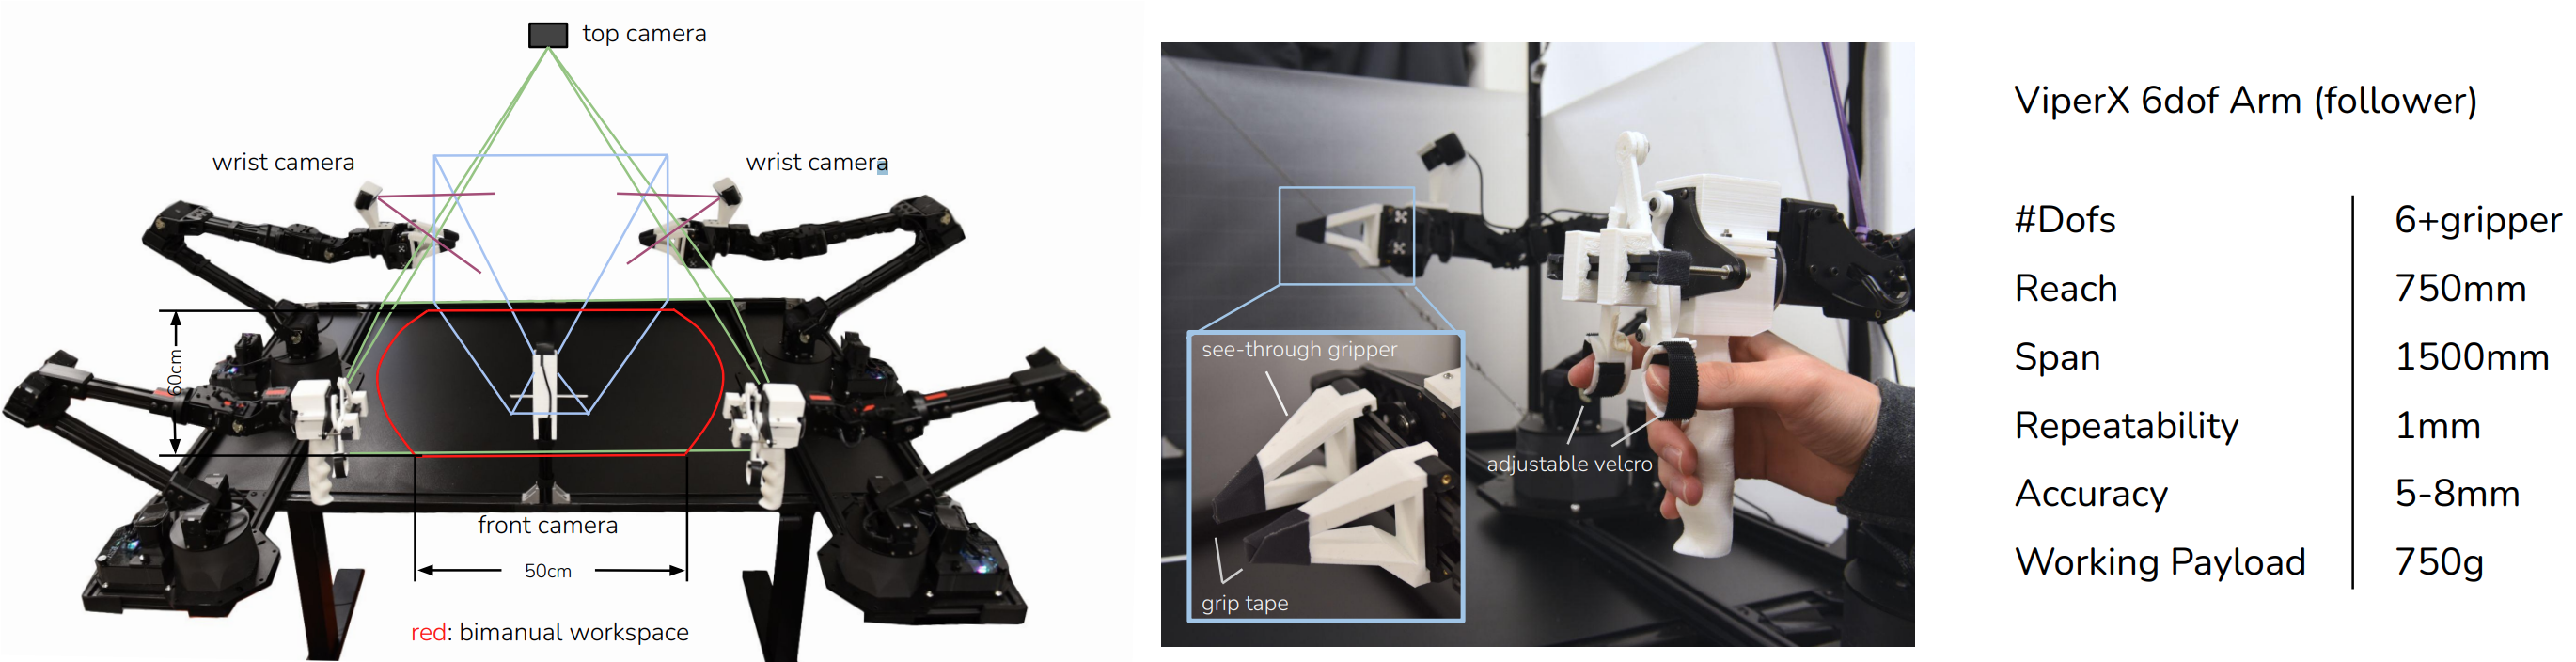
\includegraphics[width=1.0\textwidth]{./img/aloha_hw.png}
    \end{center}
    \begin{itemize}[label=-]
        \item joint-space mapping between smaller robot (windowX) to ViperX (6-DOF) vs VR headset
        % ik fails in fine-grained manipulation
        \item Robot Weight prevest fast motion + reduces joint jitter 
        \item "handle and scissor" mechanism gives continuous gripping vs binary
        \item 4x cameras: 2 wrist, one otop, one front
        \item Total hardware cost $\leq$ 20k (compare with 50k)
        \item 
    
    \end{itemize}
\end{frame}

\begin{frame}{Thank you!}
	\begin{center}
        Have a great rest of your Day!!!
	\end{center}
	\begin{center}
		% \textbf{Slides:} {\small \url{https://cs.purdue.edu/homes/jsetpal/slides/dnc_by_agop.pdf}}
	\end{center}
\end{frame}


\end{document}